\documentclass[11pt]{article}
\usepackage[a4paper, margin=20mm]{geometry}
 

\usepackage{amsmath}
\usepackage{physics}

\usepackage{graphicx}
\graphicspath{ {./figs/} }
\usepackage{subfig}

%\renewcommand{\baselinestretch}{2}
\usepackage{setspace}
\doublespacing
\usepackage{titlesec}
\usepackage{authblk}
\usepackage{titling}
\usepackage[backend=biber,
style=authoryear,
citestyle=apa]{biblatex}
\addbibresource{Reference.bib} % The filename of the bibliography

\usepackage{enumitem}

\titlespacing\section{0pt}{0pt plus 0pt minus 0pt}{0pt plus 2pt minus 2pt}
\titlespacing\subsection{0pt}{0pt plus 4pt minus 2pt}{0pt plus 2pt minus 2pt}
\titlespacing\subsubsection{0pt}{0pt plus 4pt minus 2pt}{0pt plus 2pt minus 2pt}



\begin{document}

\begin{titlepage} % Suppresses displaying the page number on the title page and the subsequent page counts as page 1
	\newcommand{\HRule}{\rule{\linewidth}{0.5mm}} % Defines a new command for horizontal lines, change thickness here
	
	\center % Centre everything on the page
	
	%------------------------------------------------
	%	Headings
	%------------------------------------------------
	
	\textsc{\LARGE University of Oxford}\\[1.5cm] % Main heading such as the name of your university/college
	
	\textsc{\Large Engineering Science}\\[0.5cm] % Major heading such as course name
	
	\textsc{\large 4YP Report}\\[0.5cm] % Minor heading such as course title
	
	%------------------------------------------------
	%	Title
	%------------------------------------------------
	
	\HRule\\[0.4cm]
	
	{\huge\bfseries The Future of Work}\\[0.4cm] % Title of your document
	
	\HRule\\[1.5cm]
	
	%------------------------------------------------
	%	Author(s)
	%------------------------------------------------
	
	\begin{minipage}{0.4\textwidth}
		\begin{flushleft}
			\large
			\textit{Author}\\
			Terence \textsc{Tan} % Your name
		\end{flushleft}
	\end{minipage}
	~
	\begin{minipage}{0.4\textwidth}
		\begin{flushright}
			\large
			\textit{Supervisor}\\
			Dr. Michael A \textsc{Osborne} % Supervisor's name
		\end{flushright}
	\end{minipage}
	
	% If you don't want a supervisor, uncomment the two lines below and comment the code above
	%{\large\textit{Author}}\\
	%John \textsc{Smith} % Your name
	
	%------------------------------------------------
	%	Date
	%------------------------------------------------
	
	\vfill\vfill\vfill % Position the date 3/4 down the remaining page
	
	{\large\today} % Date, change the \today to a set date if you want to be precise
	
	%------------------------------------------------
	%	Logo
	%------------------------------------------------
	
	\vfill\vfill
	
\includegraphics[width=0.5\textwidth]{/Users/terencetan/Documents/Uni stuff/Engineering Science/4YP/4YP-The-Future-of-Work/Report/Figures/logo.png}\\[1cm] % Include a department/university logo - this will require the graphicx package
	 
	%----------------------------------------------------------------------------------------
	
	\vfill % Push the date up 1/4 of the remaining page
	
\end{titlepage}



\section{Introduction}
\label{sec:Introduction}

\subsection{Ageing Population}
\label{subsec:ageingpopulation}

The world population is ageing over the next few decades (\cite{science}). The rising elderly to working age population ratio is increasing and will continue to do so (\cite{WHO}). This trend is known as an ageing population, and will strain the public and social services of many countries around the world (\cite{publicservicesstrain}). As one of the key social challenges facing the world for the next few decades, it would be interesting to examine how an ageing population will affect the economy, and in particular, the job market and the interplay with automation in the workplace. As more workers age out of the workforce, automation is expected to make up for it (\cite{futureofemployment}).

\subsection*{Related Works}


\subsection{Project Overview}
\label{subsec:projectoverview}
In this project, we aim to examine the relationship between the age distribution within occupations and the degree of automation (\cite{futureofemployment}) of those occupations. Although similar work has been done on this topic (\cite{twinthreats}), the study only looked at broad categories of employment. In this project, we will zoom in to look at specific occupations. We might also look into any correlations with the skills/knowledge required for those occupations. This will all be done using the scikit-learn library\footnote{https://scikit-learn.org/stable/} in Python. Specifically, we will look at a Bayesian non-parametric machine learning technique known as Gaussian Process (\cite{GaussianProcess}); this model was used in previous work (\cite{futureofemployment}), and so, would be a good model to start with. We will test and validate against different models and pick the best performing ones.

We will be using the proportion of elderly people as a metric for measuring the `age' of occupations. We acknowledge that the definition of elderly age varies across different countries and cultures (\cite{ageingculture}), and that the ageing process varies for different people depending on a variety of factors (\cite{levine2013modeling})(\cite{hayflick2007biological}). In fact, there are studies looking into moving beyond using chronological age to define an elderly person (\cite{KotterGrhn2015})(\cite{SOTOPEREZDECELIS2018e305})(\cite{klemera2006new}). However, there are numerous issues surrounding this approach (\cite{jylhava2017biological}), such as validation of such results are often difficult (\cite{biologicalagedifficult}), resulting in little consensus on an alternative metric to chronological age. For this reason, we will stick to the conventional definition of 65 years and older as `elderly' (\cite{who2010definition})(\cite{orimo2006reviewing})(\cite{oecddata}). This definition is also convenient for us since the oldest age group featured in our datasets are 65 years and older. Hence, the metric for measuring the `age' of an occupation will be the ratio of people aged 65 years and older to the total number of people in that particular occupation. For the rest of this paper, we will refer to this metric as the Elderly Ratio.

\subsection*{Related Works}

\section{Dataset}
\label{sec:Dataset}
We used two main metrics for this project: the automatability of occupations, and the age distribution within occupations. The dataset for the former is provided in an earlier work by \cite{futureofemployment}. The latter can be found in datasets provided by the US Bureau of Labour Statistics\footnote{https://www.bls.gov} (BLS); there is one dataset for each year from 2011 to 2021. All the datasets mentioned above use the Standard Occupational Classification (SOC) to classify the occupations, which means that we can map from one dataset to the another using the SOC codes\footnote{https://www.bls.gov/soc/2018/soc\_structure\_2018.pdf}. However, it is necessary to perform some data wrangling before we can proceed with the mapping. Additionally, changes were made to the SOC in 2018, so we would have to standardise all the datasets. In the following sections, we shall examine the datasets and the required data wrangling in more detail.

\subsection{BLS Dataset}
\label{subsec: BLS}
As mentioned in Chapter \ref{sec:Dataset}, the BLS provides one dataset for each year from 2011 to 2021. The datasets from 2011 to 2019 follow the old SOC while the 2020 and 2021 ones follow the updated version. We want to standardise everything according to the updated SOC. We first label each dataset with the respective year and concatenate  all of them along the row axis; we shall refer to this concatenated dataset as the BLS dataset for the rest of the paper. A section of the BLS dataset can be seen in Figure \ref{fig:df}. Note that the numbers under the \emph{Total} and age group columns are in thousands. Furthermore, the median age is not provided for all occupations, which makes it less useful as a metric. Hence, we will not be using it in this paper.

\begin{figure}[!htb]
    \centering
    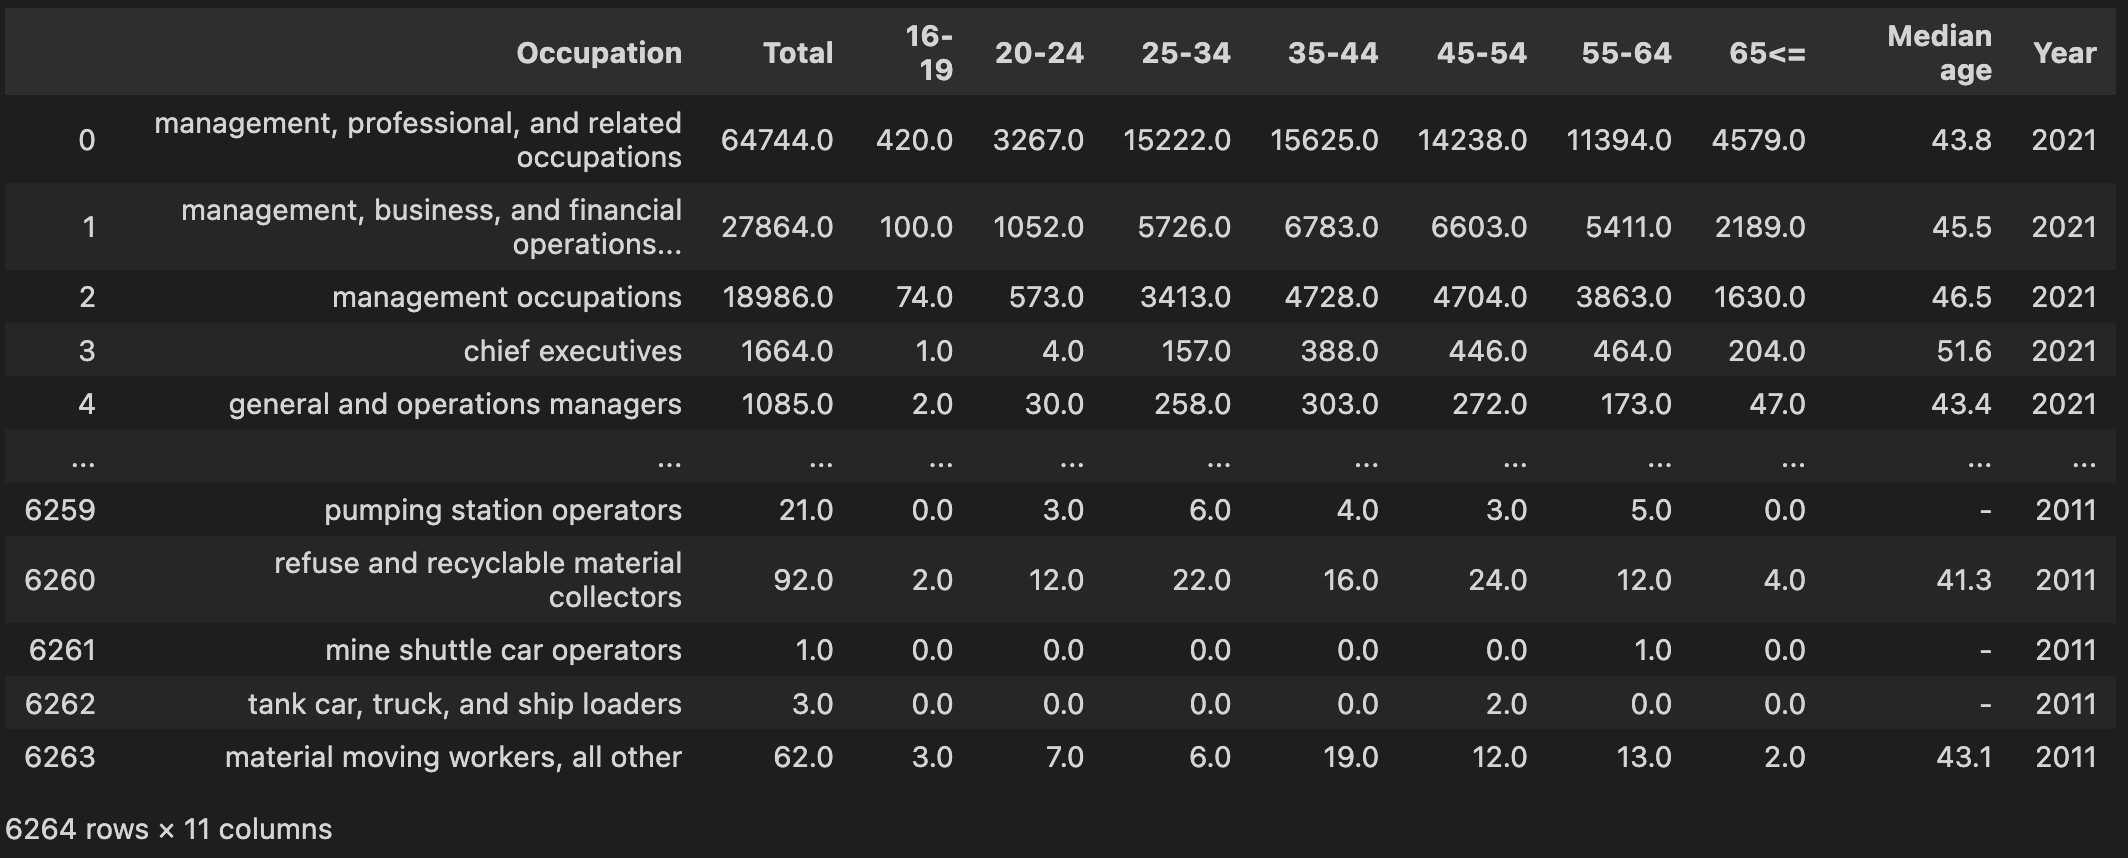
\includegraphics[width=12cm]{/Users/terencetan/Documents/Uni stuff/Engineering Science/4YP/4YP-The-Future-of-Work/Report/Figures/BLS dataset (before).png}
    \caption{BLS dataset (before processing)}
	\label{fig:df}
\end{figure}

While the BLS did provide documents\footnote{https://www.bls.gov/soc/2018/home.htm} outlining and explaining the changes to the SOC, it is generally too vague to be anything more than a rough guide. Furthermore, some of the changes made to the SOC are fairly complex. In addition to that, the BLS collected data differently for some occupations after 2019. For example, both `Marketing Managers' (SOC code: 11-2021) and `Sales Managers' (SOC code: 11-2022) are classified under `Marketing and Sales Managers' (SOC code: 11-2020). From 2011 to 2019, the BLS only collected data for `Marketing and Sales Managers' while they collected data for `Marketing Managers' and `Sales Managers' separately in 2020 and 2021. While this represents more detailed data, it is inconsistent with data collected in previous years.

In order to list out all the changes and inconsistencies, we use the \emph{pandas.DataFrame.join} function to join an old SOC dataset (from 2011 to 2019) with an updated SOC dataset (from 2020 to 2021) using the \emph{Occupation} column. We can then obtain a list of occupations from the old SOC dataset which did not join, and a corresponding list for the updated SOC dataset. We then manually go through both lists and decide on how to standardise the BLS dataset. While this process is tedious, it is reasonably doable since each list only contains about a hundred rows. The changes and rationale for them are listed alongside the occupations in both lists. All of these are placed in an Excel file\footnote{https://github.com/terencetan-c/4YP-The-Future-of-Work/blob/main/Data\%20cleaning/Changes.xlsx}.

The list of actions required are as follows: -, Delete, Change, Combine, Combine but keep. The dash indicates that no action is required. `Delete' means to delete the occupation; this is usually because the particular occupation no longer exists under the new SOC. `Change' indicates a name change. `Combine' indicates that two or more occupations should be combined into the overarching occupation. For example, the two occupations mentioned before, `Marketing Managers' and `Sales Managers', will be combined into `Marketing and Sales Managers' to ensure consistency in the BLS dataset across the years. This will basically be an element-wise addition of the rows, involving only the \emph{Total} and age group columns. This is another reason why we dropped the \emph{Median age} column since we have no way of combining median values for the BLS dataset. Lastly, the `Combine but keep' action is used in cases where we have to combine to maintain consistency but are still able to preserve some granularity by keeping the original rows. For example, the old SOC classifies the four occupations `Home Health Aides' (31-1011), `Psychiatric Aides' (31-1013), `Nursing Assistants' (31-1014), and `Orderlies' (31-1015) under `Nursing, Psychiatric, and Home Health Aides' (31-1000 and 31-1010). Additionally, the old SOC also has `Personal Care Aides' (39-9020 and 39-9021) classified separately. The new SOC renamed `Nursing, Psychiatric, and Home Health Aides' to `Home Health and Personal Care Aides; and Nursing Assistants, Orderlies, and Psychiatric Aides' (and changed the SOC code from 31-1000 to 31-1100) and moved `Personal Care Aides' (now 31-1122) under this newly named occupation. Another thing to note is that the datasets following the old SOC only collected data of `Nursing, Psychiatric, and Home Health Aides' as a whole instead of the four occupations individually. They also collected data for `Personal Care Aides'. On the other hand, the datasets following the new SOC collected data for the four occupations, `Home Health Aides' (now 31-1121), `Psychiatric Aides' (now 31-1133), `Nursing Assistants' (now 31-1131), and `Orderlies' (now 31-1132), and the newly moved occupation, `Personal Care Aides', separately. Note that both groups of datasets have data of `Personal Care Aides' on its own, and we would like to keep it that way to preserve granularity of the data. For the datasets following the old SOC, we would apply `Combine' on `Nursing, Psychiatric, and Home Health Aides' (effectively just a name change in this case) and `Combine but keep' on `Personal Care Aides'. For the new SOC datasets, we apply `Combine' on the four occupations and `Combine but keep' on `Personal Care Aides'. This way, we end up with data for a combined `Nursing, Psychiatric, and Home Health Aides' to `Home Health and Personal Care Aides; and Nursing Assistants, Orderlies, and Psychiatric Aides', while simultaneously still retaining `Personal Care Aides'.

Having systematically gone through all the inconsistencies and indicating one of the five actions required for the inconsistencies, we then use Python to automate the standardisation process. This gives us the standardised BLS dataset.

One more thing to note is that the occupations in the BLS dataset are not labelled with their respective SOC codes. This is easily rectified once the above data wrangling is completed by joining (on \emph{Occupation}) the BLS dataset with the list of SOC codes to map from occupation name to code.

\section{Preliminary Findings}
In order to make sense of how well the BLS dataset represents the US labour force, we plot the ratio of the total labour numbers provided by the BLS dataset for each year to the total US civilian labour force\footnote{https://www.bls.gov/cps/cpsaat01.htm} for that year. We do that for \emph{Major Group}, \emph{Minor Group}, \emph{Broad Group}, and \emph{Detailed Occupation} separately. The resulting plots can be seen in Figure \ref{proportion}. Clearly, \emph{Major Group} occupations are most representative of the US civilian labour force, with \emph{Minor Group} being the least. Looking through the BLS dataset, this makes sense since the BLS tended to mostly collect high-level data (\emph{Major Group}) and low-level data (\emph{Broad Group} and \emph{Detailed Occupation}). Another thing to note is that many \emph{Broad Group} occupations only contain a single \emph{Detailed Occupation} which also shares the same occupation name (for example, \emph{Chief Executives}: 11-1010 and 11-1011). Hence, it is not surprising that the ratios for \emph{Broad Group} and \emph{Detailed Occupation} are so similar.

It is important to consider the fact that the US civilian labour force includes both the employed and the unemployed. In years with unusual levels of unemployment rate, the ratios will be distorted and paint a misleading picture. Indeed, we see in Figure \ref{proportion} that there is a considerable dip in the ratios in 2020 relative to other years, coinciding with the onset of the COVID-19 pandemic (\cite{covid2020unemployment})(\cite{congresscovidunemployment}). Plotting the ratios relative to the employed portion of the US civilian labour force accounts for this; as seen in Figure \ref{proportionemp}, the dip in 2020 is no longer present. We can also see that the unemployment rate did not distort the ratios significantly. Hence, our conclusion from before still holds: the \emph{Major Group} is most representative of the US civilian labour force. With that in mind, we will try to use \emph{Major Group} data as much as possible and exercise caution when using \emph{Detailed Occupation} and \emph{Broad Group} data. As for \emph{Minor Group} data, we will neglect it given its low representation of the labour force.



\begin{figure}[!htb]
	\centering
	\subfloat[Major Group]{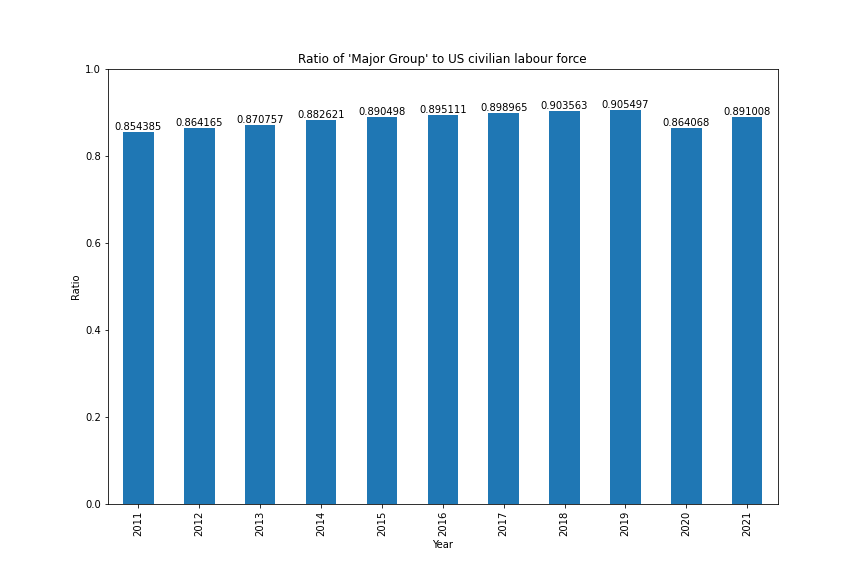
\includegraphics[width=8.5cm]{/Users/terencetan/Documents/Uni stuff/Engineering Science/4YP/4YP-The-Future-of-Work/Report/Figures/Proportion Major.png}\label{fig:promajor}}
	  \hfill
	\subfloat[Minor Group]{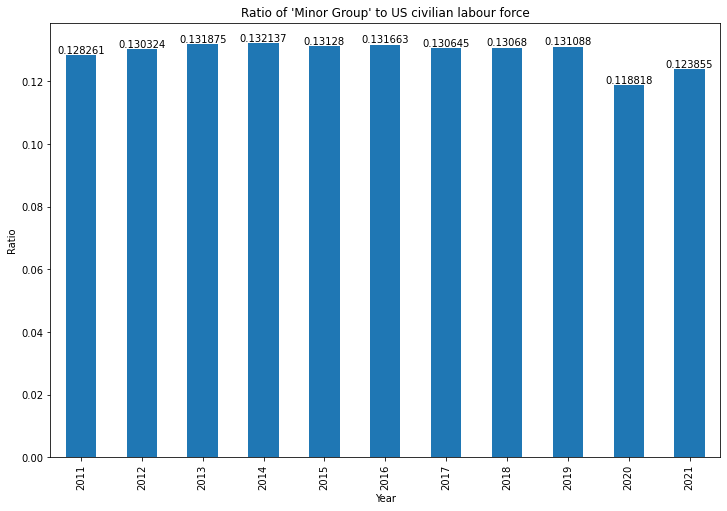
\includegraphics[width=8.5cm]{/Users/terencetan/Documents/Uni stuff/Engineering Science/4YP/4YP-The-Future-of-Work/Report/Figures/Proportion Minor.png}\label{fig:prominor}}
	\hfill
	\subfloat[Broad Group]{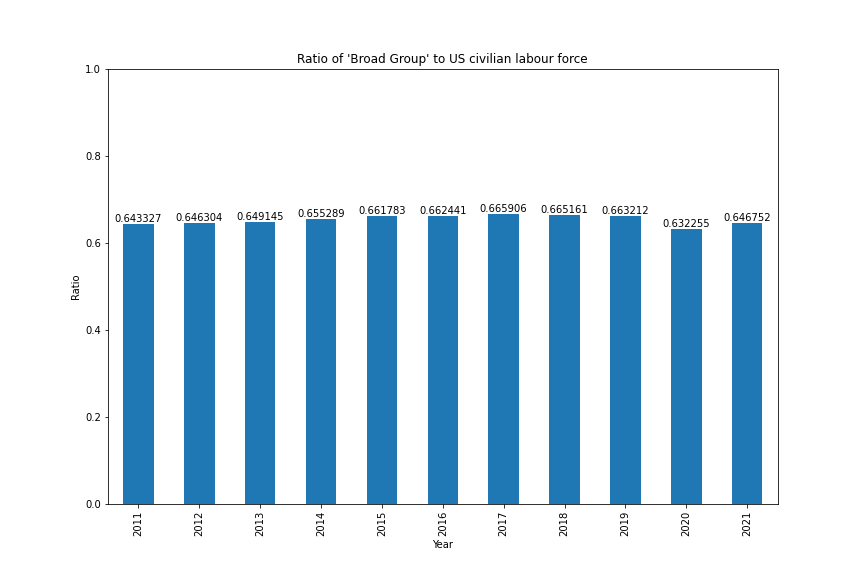
\includegraphics[width=8.5cm]{/Users/terencetan/Documents/Uni stuff/Engineering Science/4YP/4YP-The-Future-of-Work/Report/Figures/Proportion Broad.png}\label{fig:probroad}}
	\hfill
	\subfloat[Detailed Occupation]{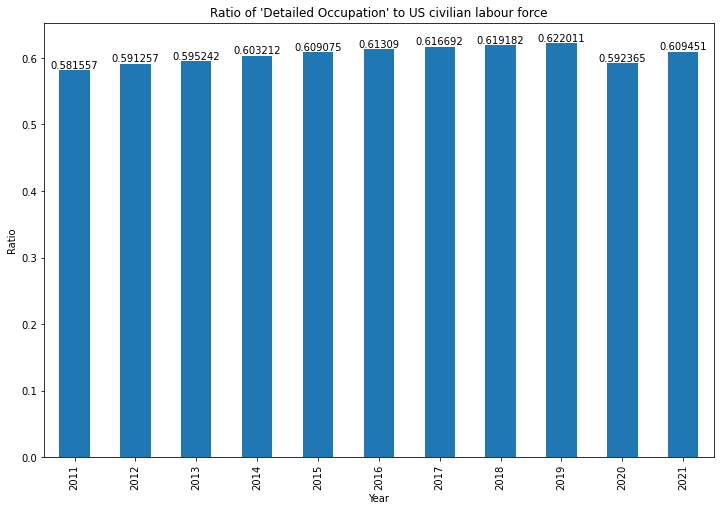
\includegraphics[width=8.5cm]{/Users/terencetan/Documents/Uni stuff/Engineering Science/4YP/4YP-The-Future-of-Work/Report/Figures/Proportion Detailed.png}\label{fig:prodetailed}}
	\hfill
	\caption{Ratio of the various SOC categories to the US civilian labour force}
	\label{proportion}
  \end{figure}
  
  \begin{figure}[!htb]
      \centering
      \subfloat[Major Group]{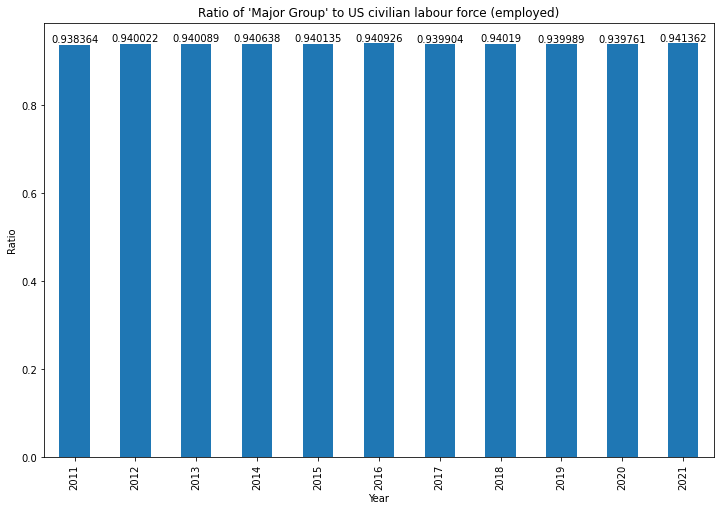
\includegraphics[width=8.5cm]{/Users/terencetan/Documents/Uni stuff/Engineering Science/4YP/4YP-The-Future-of-Work/Report/Figures/Proportion Major (employed).png}\label{fig:empmajor}}
        \hfill
      \subfloat[Minor Group]{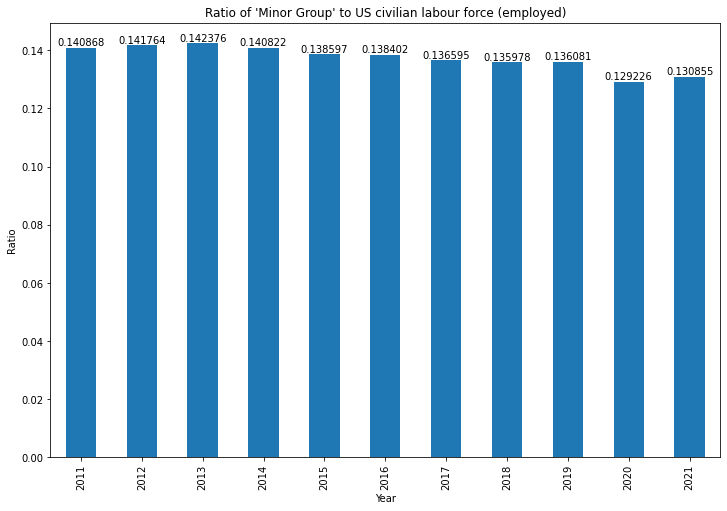
\includegraphics[width=8.5cm]{/Users/terencetan/Documents/Uni stuff/Engineering Science/4YP/4YP-The-Future-of-Work/Report/Figures/Proportion Minor (employed).png}\label{fig:empminor}}
      \hfill
	  \subfloat[Broad Group]{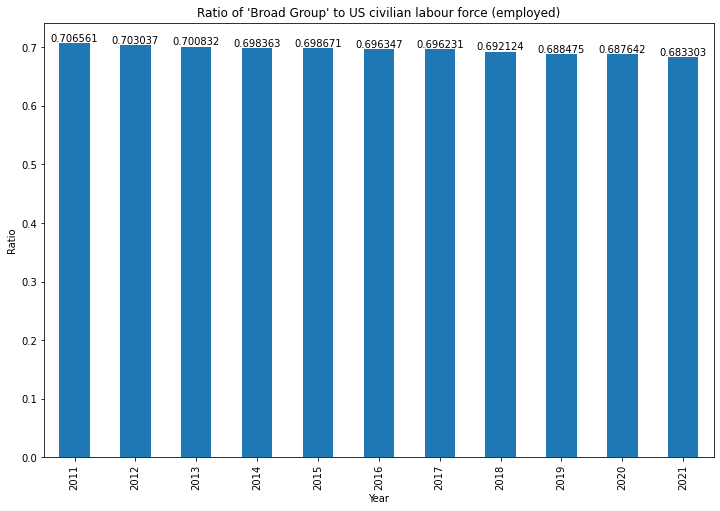
\includegraphics[width=8.5cm]{/Users/terencetan/Documents/Uni stuff/Engineering Science/4YP/4YP-The-Future-of-Work/Report/Figures/Proportion Broad (employed).png}\label{fig:empbroad}}
      \hfill
	  \subfloat[Detailed Occupation]{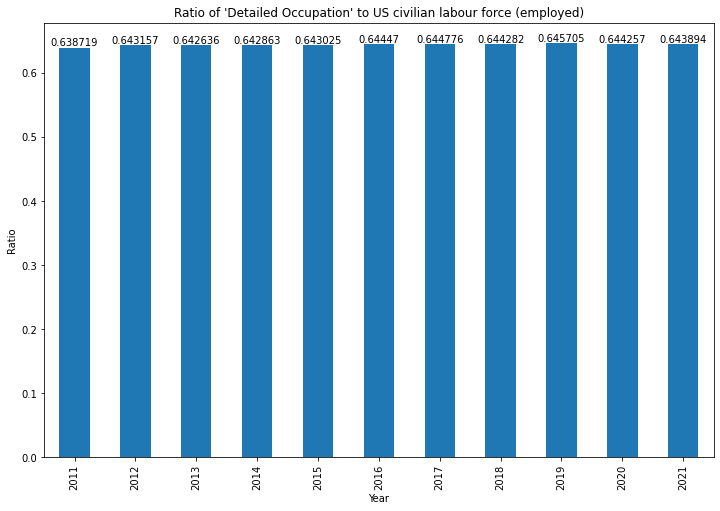
\includegraphics[width=8.5cm]{/Users/terencetan/Documents/Uni stuff/Engineering Science/4YP/4YP-The-Future-of-Work/Report/Figures/Proportion Detailed (employed).png}\label{fig:empdetailed}}
      \hfill
      \caption{Ratio of the various SOC categories to the US civilian labour force (employed)}
	  \label{proportionemp}
    \end{figure}
    
	\subsection{General Trends}
	\label{subsec:generaltrends}
	We average the Elderly Ratio (refer to Chapter \ref{subsec:projectoverview} for definition) over the Major Groups for each year, and plot the values against the years to obtain Figure \ref{fig:averageelderlyratio}. We see a steady increase over the years, which is not surprising given the ageing population of the US.

	\begin{figure}[!htb]
		\centering
		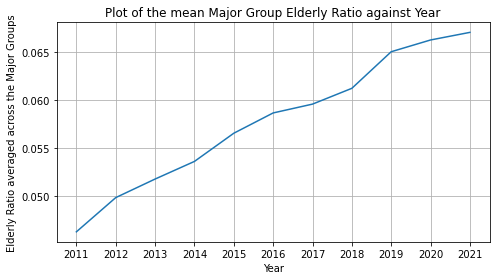
\includegraphics[width=12cm]{/Users/terencetan/Documents/Uni stuff/Engineering Science/4YP/4YP-The-Future-of-Work/Report/Figures/average major group elderly ratio.png}
		\caption{Plot of Elderly Ratio (averaged over the Major Groups) against Year}
		\label{fig:averageelderlyratio}
	\end{figure}

	We can also calculate the relative change of the Elderly Ratio for each Major Group occupation from 2011 to 2021 to obtain Figure \ref{fig:relativechange}. The `construction and extraction occupations' has the highest relative increase while the `personal care and service occupations' features the least.


	\begin{figure}[!htb]
		\centering
		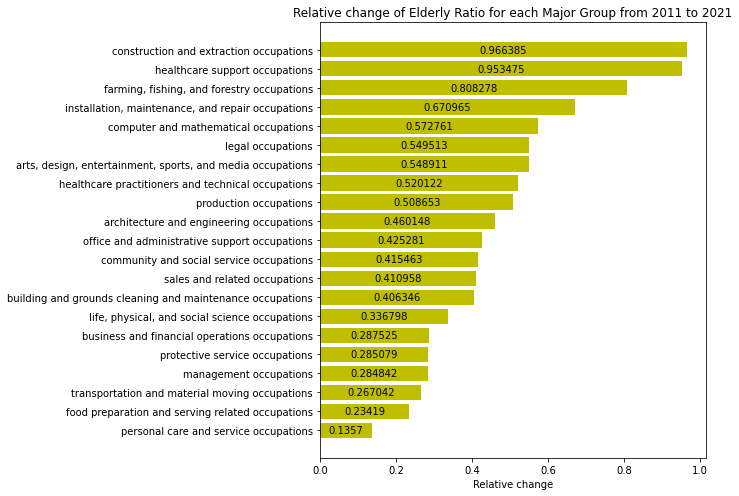
\includegraphics[width=15cm]{/Users/terencetan/Documents/Uni stuff/Engineering Science/4YP/4YP-The-Future-of-Work/Report/Figures/Relative change.png}
		\caption{Relative change of Major Groups from 2011 to 2021}
		\label{fig:relativechange}
	\end{figure}

	
\printbibliography[heading=bibintoc]


\end{document}
